\newpage
\section{Fazit}

\begin{figure}[H]
\caption{Internetnutzung weltweit}
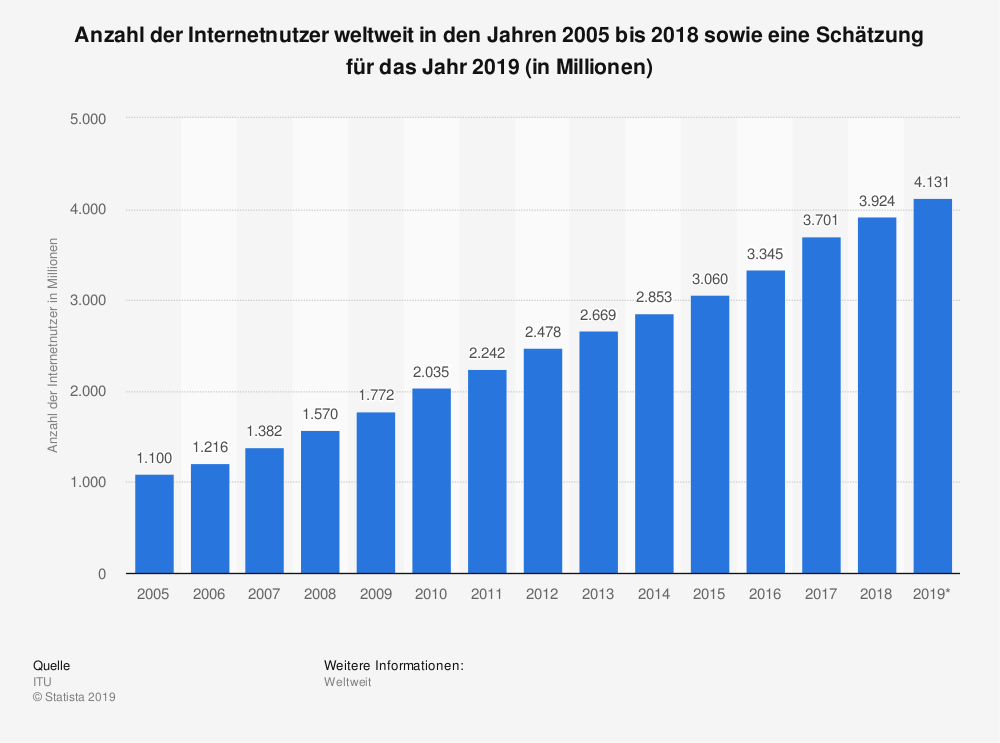
\includegraphics[width=0.8\textwidth]{stat}
\\
\cite[][27.03.2020]{Quelle: https://bit.ly/2TogWCc}
\end{figure}

Die IT Branche entwickelt sich stetig weiter. Das muss sie auch, um mit dem steigenden Wachstum mithalten zu können.

Während einige Trends schnell in Vergessenheit geraten, etablieren sich wiederrum andere als solide Optionen in der Industrie.
Grundsätzlich muss jedes Unternehmnen abwägen, ob es sich lohnt eine neue Software im Betrieb zu etablieren. Da dies immer mit Kosten verbunden ist, alleine als Zeitfaktor, 
will dies eine überlegte Investition sein.

Dazu sucht man sich Indikatoren, an denen man messen kann, ob eine Software nur ein Trend ist oder Bestand hat. Solche Indikatoren wären zum Beispiel die Zukunftsaussicht der Lösung.
Wenn eine Software von einem annerkannten bekannten Unternehmen der Branche stammt, ist das Vertrauen natürlich ein anderes als wenn ein Startup oder eine Privatperson dahinter steht.
Auch das Alter der Software und Ehrfahrungsberichte von Unabhängigen haben ein großes Gewicht im Vergleich.

Kubernetes kann einige IT Prozesse im Unternehmen vereinfachen und automatisieren, was Kosten spart. Dennoch muss das Wissen erst aufgebaut werden, somit ist dies eine Rechnung, die jedes Unternehmen
für sich machen muss. Die Frage ist nach dem ROI, dem Return-of-investment.

Was die Indikatoren angeht, kann man sagen das K8s dort sehr gut abschneidet. Wie erwähnt ist das Projekt von Google gestartet und wird seit je her auch von ihnen weiterentwickelt.
Man weiß, dass Google Kubernetes für ihre eigenen Services einsetzt, und auch K8s als Managed Service, als Software as a Service (Saas) Lösung in ihrer Cloud Platform anbietet.
Darüber hinaus setzen sehr viele der großen Unternehmen auf die K8s Platform, wie z.B. AirBnB und Reddit. Man kann also davon ausgehen, dass die meisten dieser Unternehmen an
der Weiterentwicklung von K8s interessiert sind. Somit ist der Fortbestand kein Problempunkt.

Auch auf der Seite der Erfahrungsberichte kann Kubernetes punkten. Kubernetes würde nicht so viel Verwendung finden, würden die Unternehmen darin nicht einen Vorteil sehen.
Natürlich macht K8s nicht in jeder Umgebung Sinn. Jeder muss abwägen, wie er seine Infrastruktur aufbaut. Wenn man weiß, dass sie aber auf Dauer stetig wachsen wird,
und man auf Punkte wie Hochverfügbarkeit setzen möchte, sollte Kubernetes auf jeden Fall eine Option sein, die angeschaut werden sollte.